\chapter{Problem statement}

\section{Notation and Preliminaries}

\subsection{Transformer Language Models}

We consider transformer-based language models as defined by \cite{vaswani2017attention}. Let $\mathcal{V}$ be a vocabulary of tokens, and let $\mathbf{E} \in \mathbb{R}^{|\mathcal{V}| \times d}$ be the embedding matrix, where $d$ is the embedding dimension. For a sequence of tokens $\mathbf{x} = (x_1, x_2, \ldots, x_n)$ with $x_i \in \mathcal{V}$, the transformer model processes the sequence through $L$ layers, producing hidden states $\mathbf{h}_i^l \in \mathbb{R}^d$ for each token $i$ at each layer $l$.

The final hidden state for token $i$ is denoted as $\mathbf{h}_i^L$. The language modeling head, typically a linear layer, transforms this hidden state into logits over the vocabulary:

\begin{equation}
    \mathbf{z}_i = \mathbf{W} \mathbf{h}_i^L + \mathbf{b}
    \label{eq::lm_head}
\end{equation}

where $\mathbf{W} \in \mathbb{R}^{|\mathcal{V}| \times d}$ and $\mathbf{b} \in \mathbb{R}^{|\mathcal{V}|}$ are the weight matrix and bias vector of the language modeling head, respectively. The probability distribution over the next token is then computed using the softmax function:

\begin{equation}
    P(x_{i+1} = v | x_1, \ldots, x_i) = \frac{\exp(z_{i,v})}{\sum_{v' \in \mathcal{V}} \exp(z_{i,v'})}
    \label{eq::softmax}
\end{equation}

\subsection{Embedding Space}

We define the embedding space as the $d$-dimensional vector space containing token embeddings and hidden states. For any token $v \in \mathcal{V}$, its embedding $\mathbf{e}_v \in \mathbb{R}^d$ corresponds to the $v$-th row of the embedding matrix $\mathbf{E}$.

The Euclidean distance between vectors $\mathbf{a}$ and $\mathbf{b}$ in this space is:

\begin{equation}
    d(\mathbf{a}, \mathbf{b}) = \|\mathbf{a} - \mathbf{b}\|_2 = \sqrt{\sum_{j=1}^d (a_j - b_j)^2}
    \label{eq::euclidean}
\end{equation}

\section{Research Problems}

\begin{figure}[h]
    \centering
    \begin{minipage}{0.37\textwidth}
        \centering
        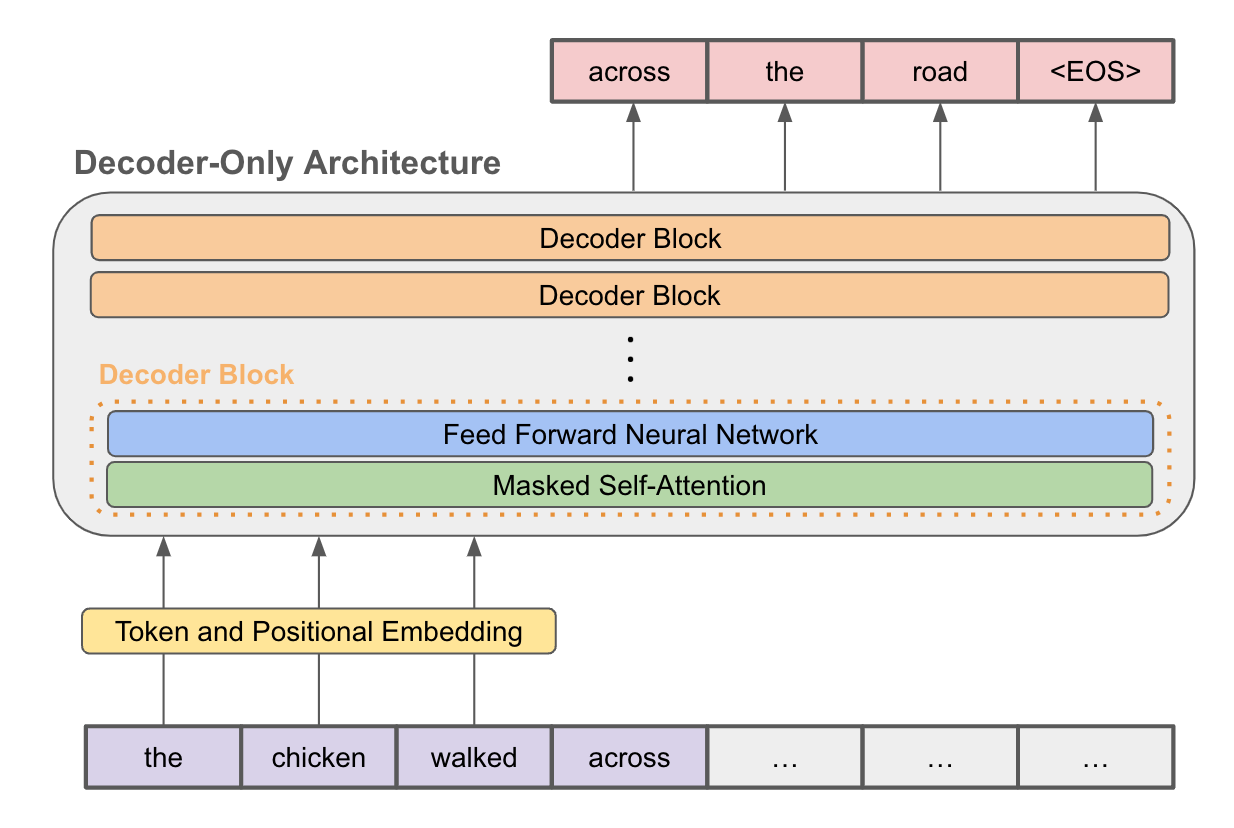
\includegraphics[width=\textwidth]{images/classic_transformer_schema.png}
        \caption{Classical illustration of the transformer schema}
        \label{fig:classic_transformer}
    \end{minipage}
    \hfill
    \begin{minipage}{0.57\textwidth}
        \centering
        \includegraphics[width=\textwidth]{images/my_transformer_schema.jpg}
        \caption{This illustration shows us the inference of the transformer as movement in the embedding space from token to token, where intermediate hidden states are denoted as intermediate steps}
        \label{fig:my_transformer}
    \end{minipage}
\end{figure}

\subsection{Reinterpreting Transformer Dynamics}

The conventional interpretation of transformer architecture, as illustrated in Figure \ref{fig:classic_transformer}, is highly technical and mechanistic. This view primarily focuses on specific matrix multiplications and how attention mechanisms combine key, query, and value vectors through various mathematical operations. While this perspective is valuable for understanding the model's implementation details, it often obscures a crucial concept: the residual stream and its evolution through the network.

We propose an alternative interpretation of transformers as performing a form of movement through embedding space, as depicted in Figure \ref{fig:my_transformer}. In this framework, the transformer's operation can be conceptualized as a trajectory in the high-dimensional embedding space, where each layer contributes to this movement in a complex, non-linear manner. Formally, we can express the evolution of the hidden state $\mathbf{h}_i^l$ for token $i$ at layer $l$ as:

\begin{equation}
    \mathbf{h}_i^{l} = \mathbf{h}_i^{l-1} + \Delta\mathbf{h}_i^{l}
    \label{eq::residual_movement}
\end{equation}

where $\Delta\mathbf{h}_i^{l}$ represents the displacement vector contributed by layer $l$. This displacement can be further decomposed into contributions from the attention mechanism and the feed-forward network:

\begin{equation}
    \Delta\mathbf{h}_i^{l} = \text{Attn}(\mathbf{h}_i^{l-1}, \mathbf{H}^{l-1}) + \text{FFN}(\mathbf{h}_i^{l-1})
    \label{eq::displacement}
\end{equation}

where $\mathbf{H}^{l-1}$ represents the set of all hidden states at layer $l-1$, and $\text{Attn}(\cdot)$ and $\text{FFN}(\cdot)$ are the attention and feed-forward network functions, respectively.

From this perspective, what attention and feed-forward layers fundamentally do in each decoder layer is shift the residual stream by a certain vector, effectively taking a step in the dynamics of the embedding space. This movement is guided by the context provided by other tokens (through attention) and by learned patterns (through the feed-forward network).

This reinterpretation of transformer operation as movement in embedding space requires empirical validation and theoretical analysis. However, if substantiated, it offers several advantages:

1. It provides a more intuitive understanding of how transformers process sequential information, viewing them as navigating through a semantic space rather than merely applying a series of transformations.

2. It establishes a connection between transformer operations and dynamical systems, potentially allowing us to apply concepts from physics and differential equations to analyze and improve these models.

3. It suggests new architectural modifications that could enhance the efficiency and interpretability of transformers by explicitly modeling the dynamics of this movement.

In the following sections, we explore this interpretation further through two specific research directions: analyzing the relationship between probability distributions and embedding distances, and developing alternative formulations of the language modeling objective based on this geometric perspective.
